\documentclass[a4paper]{usiinfbachelorproject}

\captionsetup{labelfont={bf}}
\usepackage{float}
\usepackage{amsmath}
\usepackage{graphicx}
\usepackage{enumitem}
\usepackage{booktabs}
\usepackage{hyperref}

\author{POLAD BAKHISHZADE}

\title{\textbf{LLM as Code-Correctness Judge}}
\subtitle{Unveiling the Causes of Large-Language-Model Failures when Assessing Java Code}
\versiondate{\today}

\begin{committee}
  \advisor[Università della Svizzera italiana, Switzerland]{ }{Gabriele}{Bavota}
  \coadvisor[Università della Svizzera italiana, Switzerland]{ }{Giuseppe}{Crupi}
\end{committee}

% ——————————————————————————— ABSTRACT
\abstract{
\textbf{Context.}  
Large Language Models (LLMs) are increasingly being used in software development tasks such as code generation, explanation, and bug fixing. An emerging frontier is the use of LLMs for code review—specifically, assessing whether a given implementation is functionally correct. This requires reasoning over both the specification and the code, making it a strong benchmark for code understanding.\\
\\[2pt]
\textbf{Objective.}  
This study investigates how the quality and quantity of natural-language context affect the ability of LLMs to assess code correctness. We ask: \emph{What kind of descriptive information helps or harms the model’s ability to judge whether a function is correct?}\\
\\[2pt]
\textbf{Method.}  
We extend the Java subset of the \textsc{CoderEval} benchmark by systematically enriching it with five structured documentation layers—ranging from brief summaries to formal pre/post-conditions. Each of 362 functions is paired with one correct and one incorrect candidate implementation. We then prompt three open LLMs—Qwen-0.5B, Qwen-1.5B, and DeepSeek-1.3B—to act as zero-shot code judges, under multiple prompt configurations.\\
\\[2pt]
\textbf{Findings.}  
The results reveal that different models respond differently to added context: smaller models benefit from concise behavioral descriptions but often degrade when presented with verbose examples or formal constraints. In contrast, larger models leverage detailed descriptions to reduce mistakes and achieve more reliable judgments. Some layers, such as examples, can introduce confusion and accuracy drop depending on the model.\\
\\[2pt]
\textbf{Outcome.}  
The study highlights the importance of model-specific prompt design and shows that more documentation is not always better. These insights can inform future systems that rely on LLMs for code quality assessment.\\
\\[2pt]
\textbf{Keywords}: LLMs; Code Review; Code Correctness; Prompt Engineering; Evaluation; Java; Dataset Enrichment
}

\begin{document}
\maketitle
\tableofcontents\newpage

% ——————————————————————————— 1 INTRODUCTION
\section{Introduction}\label{sec:intro}
Large Language Models (LLMs) such as ChatGPT~\cite{openai2023chatgpt}, GitHub Copilot~\cite{githubcopilot}, and StarCoder~\cite{li2023starcoder} have become widely adopted in software development workflows. Originally developed for general language understanding, these models have rapidly gained traction in code-related tasks, including code generation, explanation, repair, and synthesis~\cite{jiang2024survey, chen2021codex, wang2023codet}. Researchers are increasingly exploring the use of LLMs for tasks such as debugging, static analysis, and functional correctness evaluation.\\
\\[2pt]
Among the many challenges in this space, one particularly important question is whether LLMs can serve as reliable evaluators of automatically generated code. In industrial settings, such as at Google, the proportion of code written or assisted by machine learning systems is steadily increasing. However, verifying the correctness of such code remains an open problem. Traditional techniques like writing unit tests are time-consuming and require substantial human effort, creating a bottleneck in workflows that rely heavily on automated code generation. Existing automatic evaluation metrics—such as BLEU~\cite{papineni2002bleu}, ROUGE~\cite{lin2004rouge}, METEOR~\cite{banerjee2005meteor}, and BERTScore~\cite{zhang2019bertscore}—have shown significant limitations in this setting. These metrics often rely on reference implementations, which may not be available, and struggle to capture functional equivalence between semantically correct but syntactically different solutions. Recent studies also highlight flaws in applying embedding-based metrics to code-related tasks~\cite{naik2024limitations}. This motivates the need for oracle-free evaluation mechanisms capable of assessing whether a candidate implementation adheres to a given specification.\\
\\[2pt]
While LLMs have shown strong performance in code generation, an open question remains: can they also reason about the correctness of code? This question has received relatively little attention so far, as most benchmarks are designed for code generation. Moreover, adapting code generation benchmarks for correctness evaluation is not trivial. Many such benchmarks provide only minimal or vague natural language descriptions, which are insufficient to test whether a model understands the functionality of the implementation it is evaluating.\\
\\[2pt]
In this work, we investigate how the judging abilities of LLMs vary with the depth and completeness of the instructions provided. Specifically, we create a correctness evaluation benchmark by extending the \textsc{CoderEval} dataset with five levels of natural language documentation. These range from a simple one-line summary of the function's purpose (L1), to a high-level description of the expected behavior and edge cases (L2), an explanation of the function signature and its parameters (L3), concrete input/output examples (L4), and formal pre- and postconditions specifying what must hold before and after execution (L5). We evaluate three instruction-tuned models—Qwen-0.5B, Qwen-1.5B, and DeepSeek-1.3B—across 362 function–candidate pairs. Each pair is tested under two conditions: \emph{cumulative prompts}, where the model sees all levels from L1 up to a given level, and \emph{ablation prompts}, where a specific level (e.g., L4) is removed from the full prompt to isolate its impact.\\
\\[2pt]
Our results suggest that the ability of LLMs to utilize different types of documentation varies across models. For instance, Qwen-1.5B shows a modest improvement in accuracy from 50\% to 55\% when provided with more detailed prompts, indicating some benefit from richer context. In contrast, smaller models like Qwen-0.5B and DeepSeek-1.3B exhibit inconsistent performance, sometimes declining with additional information. These findings suggest that prompt design can influence model performance, but its effectiveness varies: while richer prompts help some models slightly, others show inconsistent or even worse results.

\subsection*{Report structure}

Section~\ref{sec:related} reviews related literature.  
Section~\ref{sec:design} presents our study design and dataset enrichment pipeline.  
Section~\ref{sec:results} covers results from cumulative and ablation experiments.  
Section~\ref{sec:concl} concludes and outlines future directions.

% ——————————————————————————— 2 RELATED WORK
\section{Related Work}\label{sec:related}
As Large Language Models (LLMs) gain traction in software development, a growing body of research is investigating their potential not only as code generators but also as autonomous evaluators. Yet, assessing whether a model can reliably judge the correctness of code remains an open and challenging question. This section presents an overview of related efforts, focusing on the current limitations of LLM-based evaluation and recent benchmark development.\\
\\[2pt]
A key concern raised by recent work is that LLMs often lack deep semantic understanding of their own outputs. West et al.~\cite{west2023generative} formulate this as the “Generative AI Paradox”: models that generate impressive solutions may still fail to understand them. Their findings show that even top-tier LLMs frequently make overconfident yet incorrect predictions, especially on reasoning-intensive tasks. Gu et al.~\cite{gu2024counterfeit} expand this concern in the coding domain. They construct “counterfeit” solutions—plausible-looking but incorrect code—and show that LLMs often fail to flag these as erroneous. Instead, models are easily misled by surface-level cues and rarely recover from their own failures. Collectively, these studies highlight a core insight: evaluating code correctness is fundamentally distinct from generating code. Therefore, it is not safe to assume that a model which produces plausible-looking solutions is also a reliable evaluator of such completions.\\
\\[2pt]
Several studies have designed benchmarks to assess LLMs’ judgment ability in isolation. Zhao et al.~\cite{zhao2024codejudgeeval} introduce \textsc{CodeJudge-Eval}, a benchmark where LLMs must decide whether a given candidate solution is correct. The dataset includes subtle bugs, edge cases, and misleading code snippets. Across 12 models, including GPT-4 and Claude, accuracy remained low—rarely exceeding 60\%, with GPT-4 reaching at most 65\%. These results suggest that current models struggle with code correctness as a task, regardless of their size. Zhao et al. highlight that even advanced models like GPT-4 frequently misclassify incorrect solutions that contain subtle bugs or misleading logic. They suggest that reformulating the task—by giving more precise and complete descriptions of the expected behavior—and training models using datasets that include both correct and incorrect implementations could help improve judgment accuracy.\\
\\[2pt]
An influential approach is introduced by ICE-Score from Zhuo~\cite{zhuo2023icescore}, which suggests using GPT-3.5-turbo to evaluate candidate implementations using precisely crafted prompts that focus on properties such as correctness and readability. The study shows that prompting the model to explain its reasoning before delivering a final judgment enhances alignment with human evaluations.\\
\\[2pt]
Expanding on this idea, Tong and Zhang~\cite{tong2024codejudge} develop \textsc{CodeJudge}, a framework that builds on ICE-Score’s principles through a structured, multi-step evaluation process. In this setup, two instruction-tuned models are guided through reasoning stages—including explanation and justification—before returning a binary decision on correctness. Experiments reveal significant improvements in judgment accuracy across five datasets and programming languages, particularly for smaller models like Llama-3-8B-Instruct. In our study, we build on these insights but take a different angle: instead of structuring the reasoning steps, we structure the task description itself. By layering increasingly rich information—ranging from summaries to behavioral specifications and input/output examples—we investigate whether more detailed descriptions help models act as better judges.\\
\\[2pt]
While the studies above focus on correctness, others explore how to align model judgments with human coding preferences. Weyssow et al.~\cite{weyssow2024codeultrafeedback} introduce \textsc{CodeUltraFeedback}, a dataset of 10,000 coding problems, each answered by 14 different LLMs. These outputs are then ranked by GPT-3.5 across five dimensions: style, readability, instruction-following, complexity, and explanation. The authors use these rankings as training data to fine-tune CodeLlama-7B-Instruct, teaching it to prefer responses that GPT-3.5 rated more highly. The fine-tuned model is evaluated on HumanEval+~\cite{lzi2023humanevalplus}, where it outperforms the original base model in both preference alignment and functional accuracy. Although the task focuses on stylistic and qualitative assessment rather than functional correctness, the results suggest that training with ranked outputs can guide LLMs to better evaluate and generate code along desired dimensions such as style and readability.\\
\\[2pt]
A complementary line of research examines LLMs in educational settings. Koutcheme et al.~\cite{koutcheme2025evaluating} assess whether LLMs can generate and evaluate feedback on student code submissions in introductory Python assignments. Their goal is to explore how models can assist in automated grading systems that support student learning. They find that open-source models like StarCoder2 perform competitively with proprietary models such as GPT-4, particularly when provided with annotated student submissions that include instructor-written feedback, which serve as exemplars for what good feedback should contain. While not directly focused on correctness classification, this work supports the broader feasibility of using LLMs as evaluators of code quality.\\
\\[2pt]
In summary, the field is converging on the idea that LLMs can act as judges, but only under carefully crafted conditions. While prior work has focused on benchmarks, multi-step reasoning, or feedback alignment, our study lies in incrementally enriching the prompt descriptions and examining how models with different sizes respond to varying levels of contextual detail when judging code correctness.

% ——————————————————————————— 3 STUDY DESIGN
\section{Study Design}\label{sec:design}

\subsection*{Research question}
\noindent\textbf{RQ –} \emph{To what extent does the quality and depth of natural language documentation affect the ability of LLMs to judge the correctness of a given Java function?}

\subsection{Context: LLMs}\label{sec:llms}
We selected three instruction-tuned LLMs of relatively small size to simulate cost-efficient evaluation scenarios: \textbf{Qwen2.5-Coder-0.5B-Instruct} and \textbf{Qwen2.5-Coder-1.5B-Instruct}~\cite{qwen2024repo}, both from Alibaba’s Qwen family, and \textbf{DeepSeek-Coder-1.3B-Instruct}~\cite{deepseek2024repo}. These models are available on Hugging Face and optimized for multi-turn interaction with structured task prompts. Each model was prompted in identical conditions, across five enrichment levels and multiple ablation runs, to evaluate how their judgment accuracy evolved as more semantic information was added—or selectively removed—from the prompt.

\subsection{Context: Dataset}\label{sec:dataset}
Our base dataset is the publicly available Java subset of the \textsc{CoderEval} benchmark~\cite{coderEval2023}, a manually verified corpus of real-world Java functions with associated candidate implementations. We started with 230 function IDs and removed 49 based on prior TA-provided exclusion criteria (e.g., functions that were duplicates, ambiguous, or noisy), ending with 181 valid functions. Each function includes the original code, a natural language docstring, and a human-assigned correctness label. However, in its raw form, \textsc{CoderEval} is generation-focused and lacks structured documentation layers. We therefore augmented each instance with a richer, five-part description to enable code understanding evaluation.

\subsection{Data Collection}\label{sec:collection}

\subsubsection{Augmenting the code generation dataset}\label{sec:augmentation}
To transform \textsc{CoderEval} from a code generation benchmark into a code understanding benchmark, we enriched each Java function with a multi-level natural language description. This transformation was performed using GPT-4o, guided by a custom prompt that forced the model to output structured information in five distinct documentation layers:
\begin{enumerate}[leftmargin=15pt]
  \item[\textbf{L1}] \textbf{Summary}: a concise one-sentence description of the function's high-level purpose, strictly excluding edge cases.
  \item[\textbf{L2}] \textbf{Behavioral description}: a 1--2 sentence narrative detailing the function’s logic, including how edge cases and special conditions are handled.
  \item[\textbf{L3}] \textbf{Signature explanation}: structured tags describing the meaning of each parameter and the return value (\texttt{@param}, \texttt{@return}, \texttt{@throws}), if applicable.
  \item[\textbf{L4}] \textbf{Examples}: several one-line input–output pairs with explanatory notes clarifying expected behavior.
  \item[\textbf{L5}] \textbf{Preconditions and postconditions}: short logical statements capturing required input constraints and expected output guarantees.
\end{enumerate}
The input to GPT-4o consisted of the full function body and its name, and the output was strictly constrained to follow the five-part format with no extra commentary or filler tokens. During development, multiple iterations of the prompt were tested to reduce verbosity, ensure syntactic consistency, and avoid contamination of L1 with behavioral detail.\\
\\[2pt]
Once the final prompt format was locked, we generated all five layers for the full set of 181 function IDs. We manually inspected and corrected the outputs for all rows, initially spot-checking 20–30 examples, then proceeding to a full sweep. Particular attention was paid to ensuring:
\begin{itemize}[leftmargin=12pt]
  \item L1 never included edge cases or technical terms.
  \item L2 correctly expanded the logic and covered edge behavior.
  \item L3 tags were accurate and omitted irrelevant fields.
  \item L4 examples reflected both standard and boundary behavior.
  \item L5 constraints were logically sound and matched the function logic.
\end{itemize}
After parsing the output into structured columns, the enriched dataset was stored in CSV format, ready for prompt composition.

\subsubsection{Generating the LLM’s judgments}\label{sec:judgments}
To evaluate whether LLMs can judge functional correctness from natural language descriptions, we paired each of the 181 functions with two candidate implementations: one correct and one incorrect. These implementations were selected from the official CoderEval knowledge base\footnote{\url{https://github.com/poladbachs/Bachelor-Thesis/blob/main/CoderEval/knowlbase_codereval.csv}}, which contains over 5,000 Java methods previously generated by various models.\\
\\[2pt]
We applied a strict filtering process to clean this pool and remove trivial or placeholder code. The cleaning was done using a custom script that rejected candidates based on several heuristics:
\begin{itemize}[leftmargin=12pt]
  \item Contained known placeholder phrases such as \texttt{“TODO”}, \texttt{“not implemented”}, \texttt{“assuming”}, etc.
  \item Contained only print statements or placeholder bodies, such as \texttt{System.out.println("To be implemented");}.
\item Had extremely low information density, for example: \texttt{return;} or \texttt{return 0;}.
\item Consisted of vague pseudocode or empty shells without logic, such as \texttt{/* implementation goes here */}.
\end{itemize}
For each function, we then attempted to find one correct and one incorrect candidate from the filtered KB. When multiple valid candidates existed, a random sample was selected. If no valid correct candidate was found in the KB, we used the official CoderEval reference code as a fallback. If no valid incorrect candidate was found, we either skipped the entry or, in two edge cases, manually injected incorrect candidates by rewriting a correct one into a subtly incorrect form. This process yielded a total of 362 candidate pairs (181 functions × 2), forming a balanced dataset.\\
\\[2pt]
Each of the three LLMs—Qwen-0.5B, Qwen-1.5B, and DeepSeek-1.3B—was evaluated using a consistent prompt template. The prompt contained:
\begin{itemize}[leftmargin=12pt]
  \item A fixed task instruction: "Judge whether the candidate implementation is correct given the function description."
  \item A binary output schema: 0 = incorrect, 1 = correct.
  \item One or more of the five documentation layers (L1–L5), depending on the experimental condition.
  \item The first line of the candidate function (its signature).
  \item The full candidate code.
\end{itemize}
The models were loaded via Hugging Face Transformers with the following inference settings: temperature 0.2, max\_new\_tokens 20. Prompts were fed in via the tokenizer, and the generated output was parsed to extract either \texttt{0} or \texttt{1}. Any deviations were treated as invalid predictions, outputting None. This pipeline was run across 15 incremental configurations (3 models × 5 levels), plus 8 additional ablation runs where selected layers were removed to analyze their individual contribution to accuracy. All results were logged, converted to structured CSVs, and stored for downstream analysis and visualization.


\subsection{Data Analysis}\label{sec:analysis}
We analyzed the model predictions along two experimental axes: prompt enrichment and prompt ablation.\\
\\[2pt]
In the \textbf{prompt enrichment setting}, each model was evaluated across five runs:
\[
\text{L1};\; \text{L1+L2};\; \text{L1+L2+L3};\; \text{L1+L2+L3+L4};\; \text{L1+L2+L3+L4+L5}
\]
This resulted in 15 total runs (3 models × 5 levels). We tracked confusion matrix components—true positives, true negatives, false positives, and false negatives—for each run, and computed accuracy as the primary metric.\\
\\[2pt]
We then conducted an \textbf{ablation study} with 8 additional runs. Here, we removed selected documentation levels from the full prompt, isolating their individual contribution. Importantly, the ablations were not exhaustive. Instead, we focused on levels that appeared least influential based on prior analysis—e.g., removing L4 (Examples) or L5 (Pre/postconditions). In some cases, notably with DeepSeek-1.3B, performance improved when L5 was excluded, suggesting that some prompts introduced noise or confusion rather than clarity.\\
\\[2pt]All outputs and metrics were saved as CSV files, and visualization scripts generated comparative bar plots per model. These allowed us to contrast how models responded to incremental detail versus selective removal of context.

\subsection{Replication Package}\label{sec:replication}
All source code, enriched datasets, model evaluation scripts, and plotting tools are available in the following GitHub repository:

\begin{center}
\url{https://github.com/poladbachs/Bachelor-Thesis}
\end{center}

The repository includes all CSVs, ablation results, accuracy plots, and confusion matrix visualizations. Dependencies are listed in a `requirements.txt`, and a step-by-step guide for full replication is provided in the README.


% ——————————————————————————— 4 RESULTS
\section{Results \& Discussion}\label{sec:results}

%------------------------------------------------------------------
\subsection{Incremental enrichment (L1 $\rightarrow$ L5)}
%------------------------------------------------------------------

\begin{figure}[H]\centering
  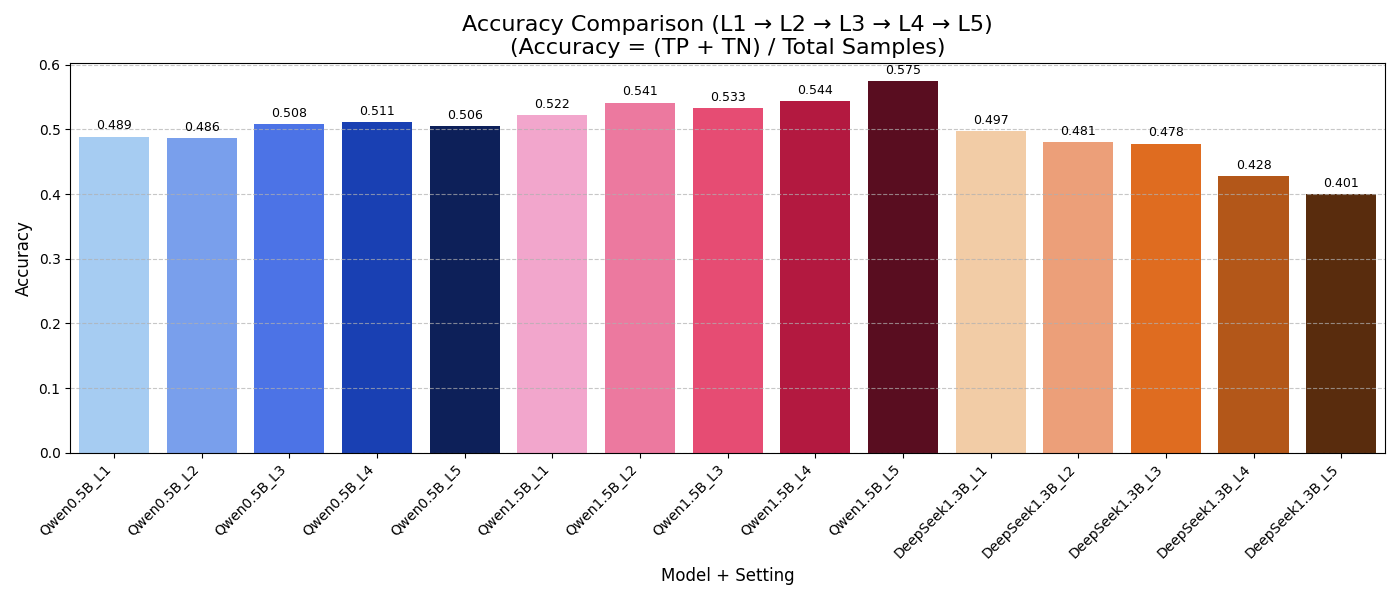
\includegraphics[width=0.95\linewidth]{figures/accuracy_comparison.png}
  \caption{Accuracy per model and documentation level.}
  \label{fig:acc-l1-l5}
\end{figure}

\paragraph*{Accuracy trends.}
We observe clear divergence in how each model responds to additional natural-language context:

\begin{itemize}[leftmargin=12pt]
  \item \textbf{Qwen-0.5B}: After stagnating on L1–L2, the model improves through L3 and L4, peaking at 0.511. L5 slightly degrades performance, suggesting diminishing returns or confusion from formal logic.
  
  \item \textbf{Qwen-1.5B}: Displays consistent benefit from each additional layer, rising steadily to 0.575 at L5. This model appears to handle verbosity well and leverages the full specification.

  \item \textbf{DeepSeek-1.3B}: Begins strong at 0.497 with minimal input, but drops with every added level—falling below 0.41 at L5. More context leads to worse performance, implying overload or poor instruction tuning for interpretive tasks.
\end{itemize}

These trends support our core hypothesis: smaller models benefit from concise cues, while larger models thrive on richer context. However, more detail is not universally helpful—its usefulness depends on model capacity and internal robustness to verbosity.

\vspace{0.8em}

% --------------------------- Qwen-0.5B
\begin{figure}[H]\centering
  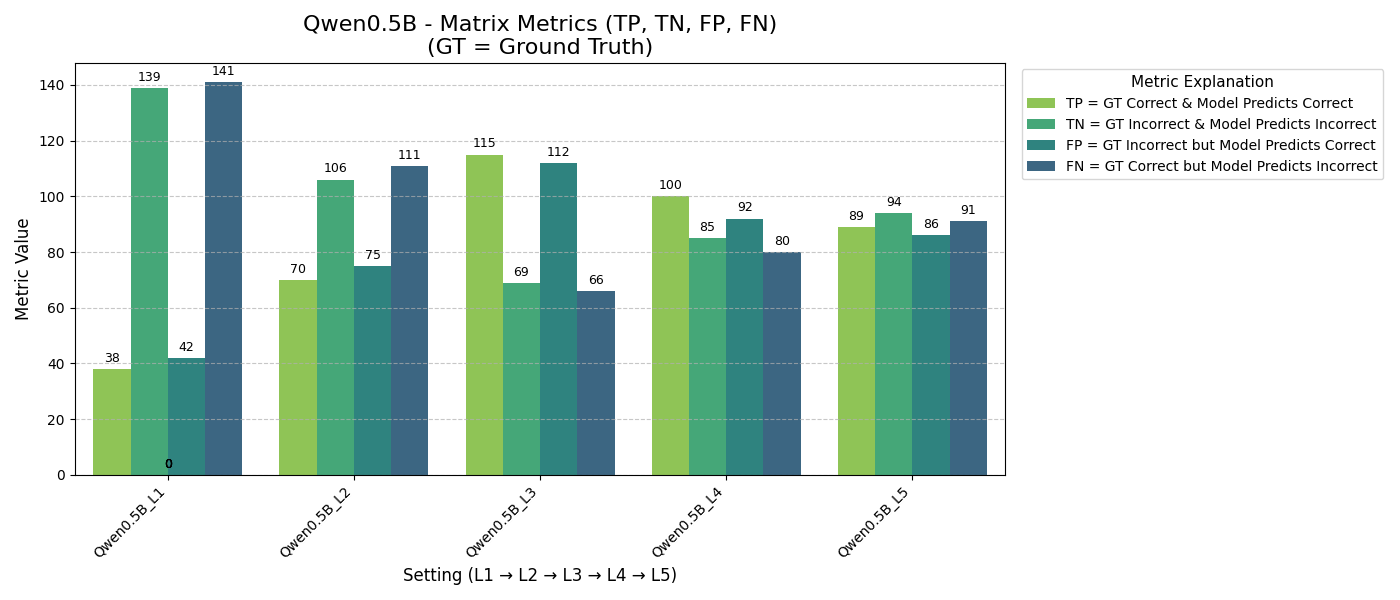
\includegraphics[width=\linewidth]{figures/Qwen0.5B_matrix_metrics.png}
  \caption{Confusion-matrix metrics — Qwen-0.5B.}
  \label{fig:q05-matrix}
\end{figure}

\paragraph*{Interpretation — Qwen-0.5B.}
Early stages (L1–L2) show a struggle to distinguish correct from incorrect implementations, with high false negatives. L3 and L4 reduce FN significantly, converting many correct cases into true positives. However, at L5 false positives creep back in, suggesting that formal conditions (pre/post) mislead the model or increase ambiguity. Overall, Qwen-0.5B needs concise clarity—too much structure destabilizes its judgment.

\vspace{0.8em}

% --------------------------- Qwen-1.5B
\begin{figure}[H]\centering
  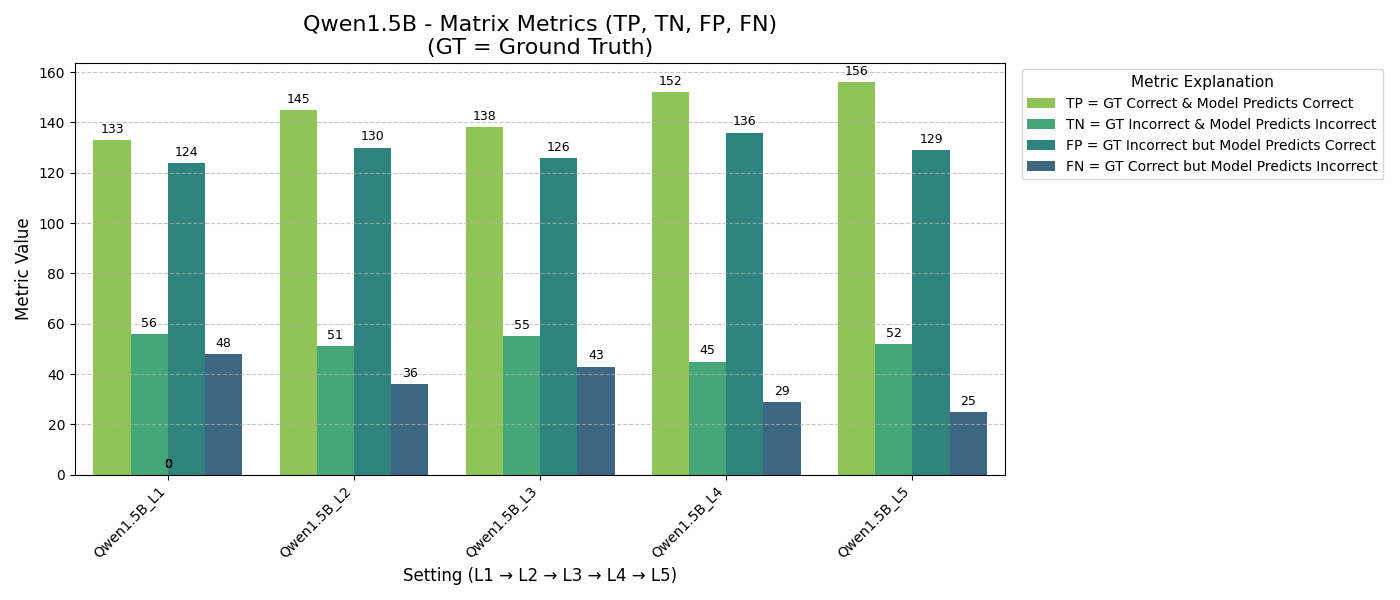
\includegraphics[width=\linewidth]{figures/Qwen1.5B_matrix_metrics.png}
  \caption{Confusion-matrix metrics — Qwen-1.5B.}
  \label{fig:q15-matrix}
\end{figure}

\paragraph*{Interpretation — Qwen-1.5B.}
The larger Qwen model handles incremental context with ease. As layers are added, false negatives drop sharply while true positives grow, especially after L4–L5. Pre/post-conditions help the model rule out wrong implementations without over-predicting correctness (FP stays stable). The balance between increased TP and maintained TN implies that Qwen-1.5B is the most context-aware model among the three.

\vspace{0.8em}

% --------------------------- DeepSeek-1.3B
\begin{figure}[H]\centering
  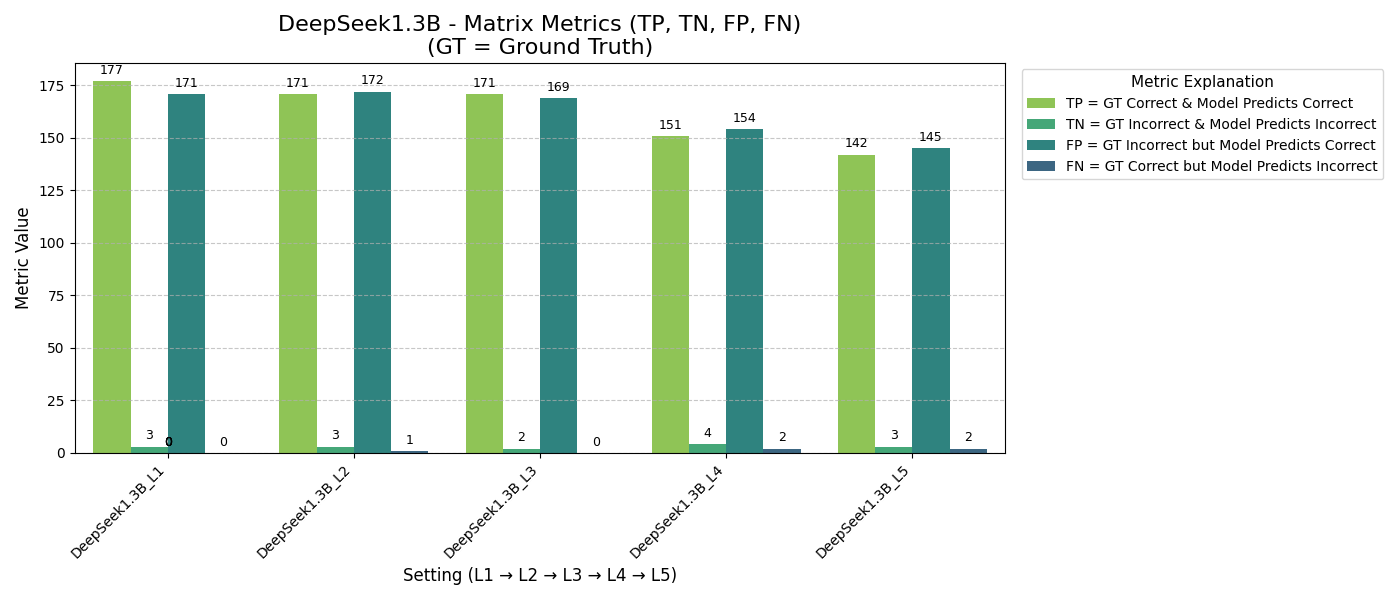
\includegraphics[width=\linewidth]{figures/DeepSeek1.3B_matrix_metrics.png}
  \caption{Confusion-matrix metrics — DeepSeek-1.3B.}
  \label{fig:ds-matrix}
\end{figure}

\paragraph*{Interpretation — DeepSeek-1.3B.}
Despite its comparable size, DeepSeek behaves like a brittle small model in judgment tasks. At L1 and L2, it achieves high TP with minimal FN. But starting at L3, false positives spike and true negatives collapse. This suggests that the added details—examples, constraints—shift attention away from core logic and confuse decision boundaries. It likely overfocuses on surface patterns in examples, falsely validating buggy code.



\subsection{Single-layer ablations}

\begin{table}[H]\centering
\caption{Accuracy after removing one layer. Values in parentheses show the change relative to the full prompt (L1--L5).}
\begin{tabular}{lccc}
\toprule
\textbf{Model} & \textbf{No L1} & \textbf{No L2} & \textbf{No L4} \\ \midrule
Qwen-0.5B  & 0.481 (–0.025) & \textbf{0.450 (–0.056)} & 0.494 (–0.012) \\
Qwen-1.5B  & 0.572 (–0.003) & 0.558 (–0.017) & 0.552 (–0.023) \\
DeepSeek-1.3B & \textbf{0.500 (+0.099)} & 0.434 (+0.034) & 0.428 (+0.028) \\
\bottomrule
\end{tabular}
\end{table}

\paragraph*{Interpretation.}
\begin{itemize}[leftmargin=12pt,itemsep=0pt]
  \item Removing behaviour (L2) cripples Qwen-0.5B (–5.6pp) $A \Rightarrow B$
 small model needs that layer.  
  \item Summary (L1) is useless or noisy for DeepSeek (+9.9pp when removed).  
  \item Qwen-1.5B tolerates all removals ($\leq$2pp), showing robustness.
\end{itemize}

\subsection{Compound ablations (illustrative)}

For space we discuss one illustrative combo per model:

\begin{itemize}[leftmargin=12pt]
  \item \textbf{Qwen-0.5B No L1 \& No L4}: accuracy 0.506 (–0.006 vs. full) — removing summary offsets example noise.  
  \item \textbf{Qwen-1.5B No L1 \& No L4}: 0.558 (–0.017) — examples help this model.  
  \item \textbf{DeepSeek No L2 \& No L4}: 0.478 (+0.078) — minimal prompt is best.  
\end{itemize}

\subsection{What makes a layer “noisy”?}
Manual error analysis highlights three patterns:

\begin{enumerate}[label=\alph*),leftmargin=15pt,itemsep=0pt]
  \item \textbf{Example bias}.  L4 lists only happy-path cases → model over-predicts “correct”.  
  \item \textbf{Narrative redundancy}.  L2 restates corner cases differently from L5, confusing alignment.  
  \item \textbf{Generic summaries}.  L1 adds little entropy; for DeepSeek it seems to trigger a “looks plausible → correct” bias.
\end{enumerate}

% ——————————————————————————— 5 CONCLUSIONS
\section{Conclusions \& Future Work}\label{sec:concl}

\begin{itemize}[leftmargin=12pt]
  \item Moderate enrichment (+behaviour, +signature) boosts small models (+8pp).  
  \item Verbose layers (examples, formal conditions) help mid-size models but harm 0.5 B and DeepSeek.  
  \item Removing noisy layers (summary or examples) can recover performance (DeepSeek +10pp).  
\end{itemize}

\textbf{Next steps}.  
\begin{enumerate}[label=\arabic*.]
  \item Fine-tune a 0.5 B checkpoint on the enriched dataset.  
  \item Auto-select minimal counter-examples to make L4 compact and balanced.  
  \item Extend to Python and larger open models (e.g.\ Llama-3-8B).  
\end{enumerate}

% ——————————————————————————— REFERENCES
\bibliographystyle{abbrv}
\bibliography{references}

\end{document}
